% fluxograma_arduino_agricultura_colorido.tex
\documentclass[border=10pt]{standalone}
\usepackage{tikz}
\usetikzlibrary{shapes.geometric, arrows.meta, positioning}

\begin{document}
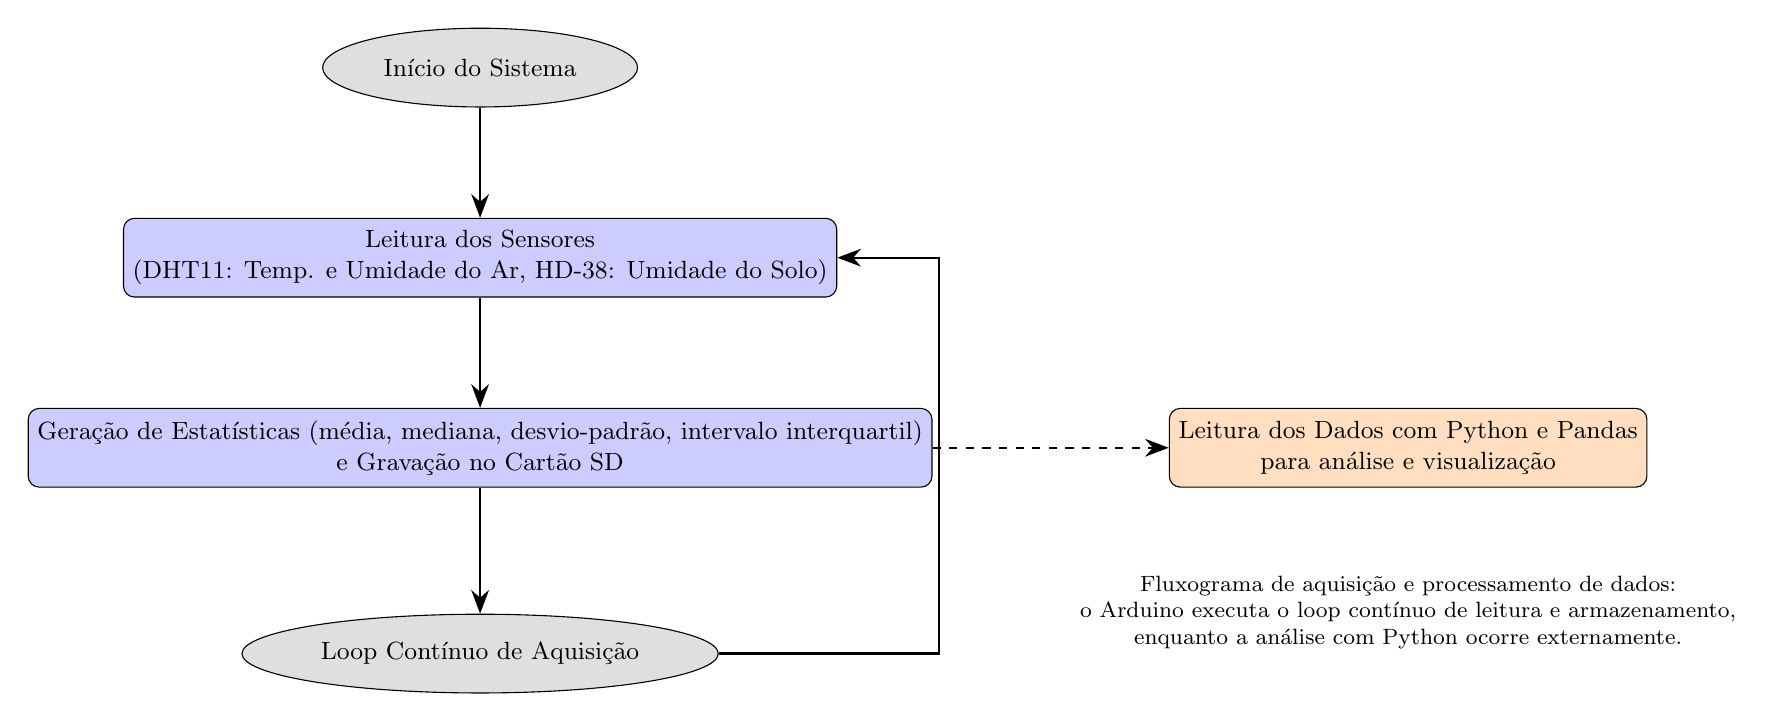
\begin{tikzpicture}[
  node distance=14mm and 25mm,
  font=\small,
  startstop/.style={ellipse, draw, fill=gray!25, minimum width=40mm, minimum height=10mm, align=center},
  process/.style={rectangle, draw, fill=blue!20, rounded corners, minimum width=50mm, minimum height=10mm, align=center},
  io/.style={trapezium, trapezium left angle=70, trapezium right angle=110, draw, fill=green!20, minimum width=50mm, minimum height=10mm, align=center},
  python/.style={rectangle, draw, fill=orange!25, rounded corners, minimum width=55mm, minimum height=10mm, align=center},
  arrow/.style={thick, -{Stealth[length=3mm]}}
]

% Nodes
\node[startstop] (inicio) {Início do Sistema};
\node[process, below=of inicio] (leitura) {Leitura dos Sensores \\ (DHT11: Temp. e Umidade do Ar, HD-38: Umidade do Solo)};
\node[process, below=of leitura] (estatistica) {Geração de Estatísticas (média, mediana, desvio-padrão, intervalo interquartil) \\ e Gravação no Cartão SD};
\node[startstop, below=of estatistica, yshift=-2mm] (loop) {Loop Contínuo de Aquisição};

\node[python, right=30mm of estatistica] (python) {Leitura dos Dados com Python e Pandas \\ para análise e visualização};

% Arrows
\draw[arrow] (inicio) -- (leitura);
\draw[arrow] (leitura) -- (estatistica);
\draw[arrow] (estatistica) -- (loop);
\draw[arrow] (loop.east) -- ++(28mm,0) |- (leitura.east); % Loop do Arduino
\draw[arrow, dashed] (estatistica.east) -- ++(25mm,0) -- (python.west); % Saída externa para Python

% Annotation
\node[align=center, below=10mm of python, font=\footnotesize] {Fluxograma de aquisição e processamento de dados:  \\ o Arduino executa o loop contínuo de leitura e armazenamento, \\ enquanto a análise com Python ocorre externamente.};

\end{tikzpicture}
\end{document}

